\documentclass[12pt,a4paper]{report}

% Packages for formatting and customization
\usepackage[utf8]{inputenc}
\usepackage{amsmath, amssymb, amsthm}
\usepackage{graphicx}
\usepackage{float}
\usepackage{hyperref}
\usepackage{geometry}
\usepackage{listings}
\usepackage{xcolor}

\definecolor{codegreen}{rgb}{0,0.6,0}
\definecolor{codegray}{rgb}{0.5,0.5,0.5}
\definecolor{codepurple}{rgb}{0.58,0,0.82}
\definecolor{backcolour}{rgb}{0.95,0.95,0.92}

\lstdefinestyle{mystyle}{
    backgroundcolor=\color{backcolour},   
    commentstyle=\color{codegreen},
    keywordstyle=\color{magenta},
    numberstyle=\tiny\color{codegray},
    stringstyle=\color{codepurple},
    basicstyle=\ttfamily\footnotesize,
    breakatwhitespace=false,         
    breaklines=true,                 
    captionpos=b,                    
    keepspaces=true,                 
    numbers=left,                    
    numbersep=5pt,                  
    showspaces=false,                
    showstringspaces=false,
    showtabs=false,                  
    tabsize=2
}

\lstset{style=mystyle}

\usepackage[toc, page]{appendix}
\usepackage{imakeidx}
\usepackage{algorithm}
\usepackage[noend]{algpseudocode}
\usepackage[T1]{fontenc}
\usepackage{booktabs}
\usepackage[backend=biber,style=numeric,doi=true,url=true]{biblatex}
\addbibresource{references.bib}
\usepackage{tikz}
\usepackage{pgfplots}
\pgfplotsset{compat=1.16}

\makeatletter
\def\BState{\State\hskip-\ALG@thistlm}
\makeatother

% Page layout
\geometry{margin=1in}


% Index creation
\makeindex


% Begin the Document
\begin{document}


% Title Page
\begin{titlepage}
  \centering
  % Insert the university logo
  
\includegraphics[width=0.45\textwidth]{Unilogo_schwarz_T3.png}\par\vspace{1.8cm}
  
  % Title and subtitle
  {\LARGE \textrm{\textbf{Matrix QM: Lanczos Algorithm Implementation for 1D Quantum Mechanics}}\par}
  \vspace{0.3cm}
  {\large \textrm{\textit{Hybrid MPI $+$ OpenMP parallelization with domain decomposition}}\par}
  \vspace{1.5cm}

% Course info
  \textbf{\normalsize Course:}\\[0.3em]
  \textrm{\normalsize Numerical Methods in Classical Field Theory and\\Quantum Mechanics (NM2b)\\[1.8em]}
  
% Authors and advisor
  \textbf{\normalsize Group Members:}\\[0.3em]
  \textrm{\normalsize Dhruv Patel (2130292)\\}
  \textrm{\normalsize Mohammadreza Khansari (2132180)\\[1.8em]}
  \textbf{\normalsize Advisor:}\\[0.3em]
  \textrm{\normalsize Dr. Tomasz Korzec\\[1.8em]}

% University and department
  \textrm{\normalsize Fakultät für Mathematik und Naturwissenschaften\\[0.3em]}
  \textrm{\normalsize Bergische Universität Wuppertal}\\[1.8em]

% Date
  {\normalsize \textrm{\today}}\par

\end{titlepage}


% Abstract
\begin{abstract}
This term paper presents a numerical framework for solving eigenvalue problems in 1D quantum mechanics using a matrix formulation and the Lanczos algorithm. Focusing on the harmonic oscillator potential, we develop serial and parallel (MPI $+$ OpenMP) versions of the algorithm that efficiently handle large, sparse Hamiltonian matrices without explicit matrix construction. The discretization scheme employs finite difference approximations for the momentum operator, enabling $O(N)$ complexity matrix-vector operations. Validation against analytical solutions of the quantum harmonic oscillator demonstrates exact agreement for low-lying energy states of the large Hermitian matrices. Parallelization strategies using domain decomposition and nearest-neighbour communication are analyzed through strong scaling tests, showing near-linear speed-up for large system sizes. The methodology provides a robust foundation for studying complex, high-dimensional quantum systems while maintaining computational efficiency through sparse matrix techniques and distributed computing.
\end{abstract}


% Table of Contents
\tableofcontents
\newpage


% Chapter 1: Introduction
\chapter{Introduction}
Quantum mechanics fundamentally describes microscopic systems through the Schrödinger equation, a partial differential equation that governs the evolution of the wave function. Although analytical solutions exist for simple potentials, such as the harmonic oscillator, most realistic systems require numerical treatment. In this work, we discretize continuous quantum operators—like momentum and position—into finite-dimensional matrices via second-order finite differences, transforming the Schrödinger equation into a matrix eigenvalue problem that is computationally tractable.

The matrix formulation becomes essential when dealing with complex potentials or scalable simulations of higher-dimensional systems, where traditional basis-set methods have limitations. However, the resulting Hamiltonian matrices surge with system size, necessitating efficient algorithms like the Lanczos method that exploit sparsity patterns and their tridiagonal structure for $O(N)$-complexity matrix-vector operations. Our implementation optimizes the quantum harmonic oscillator as a benchmark system, leveraging its known analytical solutions for validation.

For performance advancement, we extend our numerical framework to parallel computing using MPI and OpenMP. Our strategy tackles two main challenges: (1) efficiently representing sparse operators on distributed memory architectures and (2) ensuring algorithmic stability through full re-orthogonalization in parallel environments. This approach scales effectively on modern high-performance computing systems while maintaining the physical accuracy required for studying complex quantum systems.


% Chapter 2: Theory
\chapter{Theory}

\section{From Classical to Quantum Mechanics}
In classical mechanics, the dynamics of a one-dimensional system are described as:
\begin{equation}
    \frac{dx}{dt} = \frac{\partial H}{\partial p}, \quad \frac{dp}{dt} = -\frac{\partial H}{\partial x},
\end{equation}
with the Hamiltonian given by
\begin{equation}
    H(p,x) = \frac{p^2}{2m} + V(x, t).
\end{equation}
Although classical mechanics effectively describes macroscopic phenomena, it is inadequate in several key areas where quantum effects emerge:
\begin{itemize}
    \item \textbf{Atomic and Subatomic Scales:} At quantum scales, the classical picture of well-defined particle trajectories breaks down. For instance, classical mechanics inaccurately predicts stable electron orbits around nuclei, whereas quantum mechanics describes electrons as probabilistic wave functions.
    \item \textbf{Wave-Particle Duality:} Classical theory cannot reconcile the dual nature of particles (e.g., electrons, photons) exhibiting both wave-like (interference) and particle-like (localized collisions) properties.
    \item \textbf{Photoelectric Effect:} In classical wave theory, electron emission tends to depend solely on light intensity. However, experiments reveal that emission occurs only when the incident light exceeds a threshold frequency, a phenomenon accurately explained by associating photon energy with $E=h\nu$.
    \item \textbf{Relativistic Regimes:} At velocities approaching the speed of light or in strong gravitational fields, classical mechanics fails, necessitating Einstein’s theories of relativity.
\end{itemize}

Quantum mechanics replaces the deterministic framework of classical mechanics with a probabilistic description \cite{Griffiths2004Introduction, Sakurai:1341875}. The state of a quantum system is represented by a wave function $\psi(x,t)$, and physical observables are described by operators. It replaces canonical variables with operators satisfying the commutation relation $[\hat{x},\hat{p}] = i\hbar$, leading to the evolution of the system by time-dependent Schrödinger equation  as:
\begin{equation}
    i\hbar\frac{\partial}{\partial t}\psi(x,t) = \hat{H} (\hat{p}, \hat{x}) \psi(x,t),
\end{equation}
where the Hamiltonian operator $\hat{H}$ typically comprises a kinetic energy term and a potential energy term. For a one-dimensional system, the Hamiltonian operator is
\begin{equation}
\hat{H} (\hat{p}, \hat{x}) = \underbrace{\frac{\hat{p}^2}{2m}}_\textrm{kin. energy} + \underbrace{V(\hat{x}, t)}_\textrm{pot. energy},
\end{equation}
with the momentum operator defined by
\begin{equation}
p \rightarrow \hat{p} = -i\hbar\frac{d}{dx}.
\end{equation}

\section{Stationary States and Eigenvalue Problem}
When the potential $V(x)$ is time-independent, one can employ the separation ansatz $\psi(x,t) = \phi(x)e^{-iEt/\hbar}$, which transforms the time-dependent Schrödinger equation into the stationary Schrödinger equation:
\begin{equation}
    \hat{H}\phi_n(x) = E_n\phi_n(x).
\end{equation}
Here, eigenvalues $E_n$ denote the quantized energy states, and $\phi_n(x)$ are the corresponding eigenfunctions. For example, in the harmonic oscillator where $V(x) = \frac{1}{2}m\omega^2x^2$, the eigenvalues and eigenfunctions are given by
\begin{equation}
    E_n = \hbar\omega\left(n + \frac{1}{2}\right), \quad \phi_n(x) \propto H_n\left(\sqrt{\frac{m\omega}{\hbar}}x\right)e^{-m\omega x^2/2\hbar},
\end{equation}
where $H_n$ represents the Hermite polynomials.

\section{Matrix Formulation and Discretization}
For solving the Schrödinger equation numerically, the discretization is in a continuous spatial domain over a finite interval—often with periodic boundary conditions—thereby converting differential operators into matrices. Two common approaches for discretizing the second derivative (which is associated with $\hat{p}^2$) include:
\begin{itemize}
    \item \textbf{Finite Difference Method:} This approach approximates the second derivative using nearest-neighbour approximation and yields a sparse, tridiagonal matrix, with error terms proportional to $a^2$, where $a$ is the lattice spacing.
    \item \textbf{Spectral (Fourier) Method:} Constructs a dense matrix based on the spectral derivative. This method leverages the sampling theorem to reproduce continuum eigenvalues with negligible discretization error accurately \cite{doi:10.1137/1.9780898719598}.
\end{itemize}
In either case, the discretized Hamiltonian is represented as a Hermitian matrix whose eigenvalues correspond to the energy levels of the system. Discretizing space into $N$ points, where $x_k = ka$ for $k = -M, \ldots ,M$ (with periodic boundary conditions), transforms operators into matrices. For example:
\begin{itemize}
    \item \textbf{Position Operator:} Represented by the diagonal matrix $X_{kl} = x_k\delta_{kl}$
    \item \textbf{Momentum Operator:} Finite-difference approximation
    \begin{equation}
        P^2_{kl} = \frac{\hbar^2}{a^2}\begin{cases} 
        2 & k=l \\
        -1 & |k-l| = 1 \mod N \\
        0 & \text{otherwise}
        \end{cases}
    \end{equation}
\end{itemize}
Thus, the Hamiltonian matrix is given by $H = \frac{P^2}{2m} + \text{diag}(V(x_k))$, retaining the sparsity properties of the discretized kinetic term.

\section{Lanczos Algorithm for Eigenvalue Problems}
The Lanczos algorithm is an iterative method for sparse, large-scale Hermitian matrices. The process begins with a randomly initialized normalized vector $v_0$ and iteratively generates an orthonormal basis for the Krylov subspace $\mathcal{K}_k (\hat{H}, v_0) = \textrm{span}\{v_0, \hat{H} v_0, \ldots, \hat{H}^{k-1} v_0\}$, thereby reducing $\hat{H}$ to a triadiagonal matrix $T_k$. The eigenvalues of this tridiagonal matrix approximate the low-lying eigenvalues of the original Hamiltonian, and full re-orthogonalization is applied at each iteration to maintain numerical stability \cite{Higham2002}.

The efficiency of the Lanczos method arises from its reliance on matrix-vector products rather than explicit matrix storage—a critical advantage for large-scale quantum systems where the Hamiltonian is sparse. This approach generates a sequence of vectors using a three-term recurrence relation, resulting in a tridiagonal matrix whose diagonal and off-diagonal elements capture the recurrence coefficients. For systems like the harmonic oscillator, the kinetic energy operator contributes a natural tridiagonal structure (via finite differences), and the potential energy operator remains diagonal, which allows rapid computation of $\hat{H}\psi$. This combination preserves the sparsity of the overall Hamiltonian, ensuring that each iteration remains computationally tractable and can be executed in $O(N)$ operations.

Convergence of the Lanczos algorithm is typically faster for extremal eigenvalues of $T_k$, but due to rounding errors and loss of orthogonality in finite-precision arithmetic, periodic re-orthogonalization is essential. This step ensures that the generated Lanczos vectors remain mutually orthogonal, preventing spurious convergence and improving the reliability of the computed eigenvalues. Balancing numerical stability with computational efficiency is a key challenge, particularly in parallel implementations.

Parallelization of the Lanczos algorithm is achieved through domain decomposition. The wave function $\psi$ is partitioned across multiple MPI processes, with each process responsible for a segment of the spatial grid. For the harmonic oscillator, $\hat{H}\psi$ involves local stencil operations (nearest-neighbour sums), ideal for distributed computing. Additionally, OpenMP threading accelerates local operations, such as vector updates and inner products. While the orthogonalization step is inherently sequential, it leverages distributed linear algebra libraries to mitigate bottlenecks.

In practical implementations, the Lanczos algorithm \cite{Lanczos:1950:IMS} offers an efficient and scalable framework for extracting a few low-lying eigenstates from large, sparse Hamiltonians. Its iterative nature, combined with advanced parallelization techniques, makes it especially suitable for high-performance quantum mechanical simulations where only a narrow subset of the full spectrum is required. This focus on low-lying eigenstates is particularly advantageous in studies of ground-state properties requiring only a few eigenvalues and eigenvectors with low-energy excitations in quantum systems.


% Chapter 3: Numerical Methods and Parallelization
\chapter{Numerical Methods and Parallelization}

\section{Discretization Scheme}
The spatial domain is discretized as follows:
\begin{itemize}
    \item \textbf{Grid points:} $x \in \{-Ma, \ldots , -a, 0, a, \ldots , Ma\}$ with $N = 2M+1$ points,
    \item \textbf{Lattice spacing:} $a = L/N$,
    \item \textbf{Momentum discretization:} $p_n = \frac{2 \pi n}{L}$, \; $n \in -M, \ldots , +M$,
    \item \textbf{Periodic boundary conditions:} $\phi(x+L) = \phi(x)$.
\end{itemize}
Two discretization methods to approximate the kinetic energy operator $\hat{p}^2$, are:
\begin{enumerate}
    \item \textbf{Finite Difference Discretization:} The second derivative is approximated as
    \begin{equation}
    [\hat{p}^2 \psi]_i= \frac{\hbar}{a^2}\left(2\psi(x_i)-\psi(x_{i-1})-\psi(x_{i+1})\right),
    \end{equation}
    ensuring periodic boundary conditions via modular indexing.
    \item \textbf{Spectral Derivative:} The second derivative is evaluated via a discrete Fourier transform, with matrix elements
    \begin{equation}
    P^2_{kl} = \frac{\hbar^2}{N}\sum_p p^2 \cos\left(p(x_k-x_l)\right),
    \end{equation}
    which reproduces the continuum eigenvalues with minimal discretization error.
\end{enumerate}

\section{Lanczos Algorithm Implementation}
The Lanczos algorithm is implemented in Python language \cite{golub13, Press2007}. The key steps are:
\begin{itemize}
    \item \textbf{Initialization:} Begin with a random normalized vector.
    \item \textbf{Iteration:} Apply the Hamiltonian to generate a new Krylov basis vector. At each iteration, compute the diagonal ($\alpha$) and off-diagonal ($\beta$) coefficients while performing full re-orthogonalization to mitigate numerical instabilities.
    \item \textbf{Tridiagonalization:} Construct the tridiagonal matrix, whose eigenvalues approximate those of $\hat{H}$.
    \item \textbf{Eigenvalue Extraction:} Use standard routines (e.g., from \texttt{scipy.sparse.linalg} import \texttt{eigsh}, use \texttt{ARPACK}) to solve the reduced eigenvalue problem.
\end{itemize}
The iterative process generates an orthonormal basis $\{v_j\}$ that tridiagonalizes the Hermitian matrix $\hat{H}$ while preserving its spectral properties.
\begin{algorithm}
\caption{Lanczos Algorithm}\label{euclid}
\begin{algorithmic}[1]
\Procedure{Lanczos Iteration}{$m, n, a, rank, num\_procs, comm$}
    \State $sizes \gets \Call{distribute\_elements}{n, num\_procs}$
    \State $local\_n \gets sizes[rank]$
    \State $starts \gets [\,\sum_{i=0}^{p-1} sizes[i] \text{ for } p=0,\dots,num\_procs-1\,]$
    \State $start\_idx \gets starts[rank]$
    \State $M \gets \lfloor (n-1)/2 \rfloor$ \; \texttt{\# Precomputing local position array}
    \State $x\_local \gets a \cdot \text{range}(start\_idx - M,\, start\_idx - M + local\_n)$
    \State $v \gets$ zero matrix of size $(local\_n \times m)$ \; \texttt{\# Orthonormal basis}
    \State $\beta \gets$ zero vector of length $m-1$ \; \texttt{\# Off-diagonal elements}
    \State $\alpha \gets$ zero vector of length $m$ \; \texttt{\# Diagonal elements}
    \State $v_1 \gets$ random vector of size $local\_n$ \; \texttt{\# Initialize starting vector}
    \State $v_1 \gets \Call{normalize\_vector}{v_1,\, comm}$
    \State $v\_temp \gets \Call{exchange\_boundary\_data}{v_1,\, local\_n,\, rank,\, num\_procs,\, comm}$
    \State $w_1^p \gets \Call{Hv}{v\_temp,\, a,\, x\_local,\, comm}$ \; \texttt{\# First Lanczos iteration}
    \State $a_1 \gets \Call{dot\_product}{w_1^p,\, v_1,\, comm}$
    \State $w_1 \gets w_1^p - a_1 \cdot v_1$
    \State $\alpha[0] \gets a_1$
    \State $v[:,0] \gets v_1$
    \For{$j \gets 1$ to $m-1$} \; \texttt{\# Lanczos iteration loop}
        \State $\beta[j-1] \gets \Call{get\_global\_norm}{w_1,\, comm}$
        \If {$\beta[j-1] \approx 0$}
            \State $v[:,j] \gets \Call{normalize\_vector}{\text{random vector of size } local\_n,\, comm}$
        \Else
            \State $v[:,j] \gets \frac{w_1}{\beta[j-1]}$
        \EndIf
        \State $v \gets \Call{modified\_gram\_schmidt}{v,\, j+1,\, comm}$ \; \texttt{\# C kernel}
        \If {$j \bmod 10 = 0$} \; \texttt{\# Check orthogonality: every 10 iterations}
            \State $\Call{check\_orthogonality}{v,\, j+1,\, comm}$
        \EndIf
        \State $v\_tp \gets \Call{exchange\_boundary\_data}{v[:,j],\, local\_n,\, rank,\, num\_procs}$
        \State $w_1^p \gets \Call{Hv}{v\_temp,\, a,\, x\_local,\, comm}$ \; \texttt{\# C-accelerated kernel}
        \State $\alpha[j] \gets \Call{dot\_product}{w_1^p,\, v[:,j],\, comm}$
        \State $w_1 \gets w_1^p - \alpha[j]\cdot v[:,j] - \beta[j-1]\cdot v[:,j-1]$
    \EndFor
    \If {$rank = 0$} \; \texttt{\# root process}
        \State $T \gets$ tridiagonal matrix with main diagonal $\alpha$ and off-diagonals $\beta$
        \State $eigenvalues \gets$ Compute 10 smallest eigenvalues from $T$
    \EndIf
    \State \Return $eigenvalues$
\EndProcedure
\end{algorithmic}
\end{algorithm}
Re-orthogonalization at each step counteracts rounding errors, ensuring the stability and accuracy of the computed eigenvalues.

\section{Hybrid MPI+OpenMP Parallelization}
For handling large-scale simulations efficiently, the spatial domain is partitioned among MPI processes, with each process handling a contiguous block of grid points, thus holding a segment of the full wave function. OpenMP threads accelerate local computations, while MPI coordinates data exchange and global operations. Key features include:
\begin{itemize} 
    \item \textbf{Domain Decomposition:} Each MPI process holds $N/N_{proc}$ contiguous grid points.
    \item \textbf{Boundary Exchange:} Non-blocking MPI calls exchange ghost cells with neighbouring processes, ensuring that finite difference approximation for the Hamiltonian access adjacent grid points.
    \item \textbf{Collective Operations:} Global inner products and norms are computed via MPI reduction operations during the orthogonalization steps.
    \item \textbf{Overlap of Computation and Communication:} Non-blocking communications are overlapped with local computations, optimizing overall execution time. 
    \item \textbf{OpenMP Acceleration:} Critical kernels, such as the Hamiltonian application and Modified Gram-Schmidt re-orthogonalization, are implemented in C with OpenMP directives to exploit thread-level parallelism.
\end{itemize}
A pseudocode for the distributed matrix-vector product using this hybrid model is:
\begin{algorithm}
\caption{Distributed Matrix-Vector Product in Hybrid MPI$+$OpenMP}
\begin{algorithmic}[1]
\Procedure{Distributed\_MatVec}{$v_{local},\, local\_n,\, rank,\, num\_{procs}$}
    \State $right\_{rank} \gets (rank+1)\mod num\_{procs}$
    \State $left\_{rank} \gets (rank-1)\mod num\_{procs}$
    \State \texttt{\# Initiate non-blocking communication for ghost cells}
    \State \Call{MPI\_Isend}{$v_{local}[0],\, destination = left\_{rank}$}
    \State \Call{MPI\_Isend}{$v_{local}[local\_{n}-1],\, destination = right\_{rank}$}
    \State \Call{MPI\_Irecv}{$ghost\_{left},\, source = right\_{rank}$}
    \State \Call{MPI\_Irecv}{$ghost\_{right},\, source = left\_{rank}$}
    \State \Call{MPI\_Waitall}{}
    \State \texttt{\# Build extended vector with ghost cells}
    \State Set $v_{ext}[1:local\_{n}] \gets v_{local}$
    \State Set $v_{ext}[0] \gets ghost\_{left}$,\, and $v_{ext}[local\_{n}+1] \gets ghost\_{right}$
    \State \texttt{\# Apply Hamiltonian operator using OpenMP-accelerated kernel}
    \State $w_{local} \gets \Call{Hv}{v_{ext},\, a,\, x_{local},\, local\_{n}}$
    \State \Return $w_{local}$
\EndProcedure
\end{algorithmic}
\end{algorithm}

In our implementation, the Python code (using \texttt{mpi4py}) manages the MPI tasks while delegating computationally intensive parts—such as the Hamiltonian application and the Modified Gram-Schmidt process—to C kernels optimized with OpenMP. This hybrid strategy enables us to scale to larger problem sizes and significantly reduces the execution time.


% Chapter 4: Results: Strong Scaling Performance
\chapter{Results: Strong Scaling Performance}

\section{Serial Implementation}
The serial implementation employs the Lanczos algorithm to approximate the eigenvalues of a one-dimensional quantum Hamiltonian. The Hamiltonian operator is discretized using a finite difference approximation for the kinetic term in conjunction with a power-law potential. The algorithm is implemented in Python, with key routines—such as the Hamiltonian application and the Modified Gram-Schmidt reorthogonalization—optimized for efficiency. The spatial domain $x \in [-L/2, L/2]$ is discretized into $N = 2M + 1$ grid points with lattice spacing $a = L/N$. The corresponding momentum grid is defined by $p_n = \frac{2\pi n}{L}$ for $n = -M, \ldots , +M$, with periodic boundary conditions enforced.

A random normalized vector initiates the Lanczos process, which iteratively constructs an orthonormal basis of the Krylov subspace. The Hamiltonian matrix is effectively represented as a sparse tridiagonal matrix: the diagonal elements $(\alpha)$ capture the potential energy, while the off-diagonal elements $(\beta)$ correspond to the kinetic energy. Full reorthogonalization is performed at each iteration via Modified Gram-Schmidt to ensure numerical stability. The resulting tridiagonal matrix is then diagonalized using routines from (\texttt{scipy.sparse.linalg.eigsh}) to extract the ten smallest eigenvalues, serving as a foundational benchmark for assessing the algorithm’s convergence and accuracy.

We focus on the quantum harmonic oscillator, $(V(x) = \frac{1}{2}x^2)$, using the following baseline parameters:
\begin{itemize}
    \item \textbf{Grid Resolution:} $N = 153$ points over $L = 25$, yielding a lattice spacing $a = L / N \approx 0.163$,
    \item \textbf{Krylov Subspace Size:} Initially, $m = N$ (full orthogonalization); subsequent tests with fixed $m$ and increasing $N$,
    \item \textbf{Natural Units:} $\hbar = m = \omega = 1$, with analytical eigenvalues given by $E_n = n + \frac{1}{2}$.
\end{itemize}
For the baseline case $(m = N = 153)$, the Lanczos algorithm converges rapidly. The computed eigenvalues (presented in Table~\ref{tab:serial_eigenvalues}) agree closely with the analytical solutions, with relative errors below approximately $1.7\%$ for the ten smallest eigenvalues, i.e., in the order of $10^{-3}$ to $10^{-2}$. Residual norms are monitored at each iteration to ensure convergence and stability.
\begin{table}[h]
    \centering
    \caption{Computed Eigenvalues and Relative Errors (Serial Implementation)}
    \label{tab:serial_eigenvalues}
    \begin{tabular}{ccc}
    \hline
    $n$ & $E_n^{Computed}$ & $Relative\;Error$ \\ \hline
    $0$ & $0.4992$ & $-0.17\%$ \\
    $1$ & $1.4958$ & $-0.28\%$ \\
    $2$ & $2.4891$ & $-0.44\%$ \\
    $3$ & $3.4790$ & $-0.60\%$ \\
    $4$ & $4.4655$ & $-0.77\%$ \\
    $5$ & $5.4486$ & $-0.93\%$ \\
    $6$ & $6.4283$ & $-1.10\%$ \\
    $7$ & $7.4045$ & $-1.27\%$ \\
    $8$ & $8.3772$ & $-1.44\%$ \\
    $9$ & $9.3465$ & $-1.62\%$ \\ \hline
    \end{tabular}
\end{table}
To further investigate the method’s performance, we consider a fixed Krylov subspace size $m$ at its baseline value $(153)$ and increase the total number of grid points $N$ $(\text{i.e.}, \; N = 153, 307, 613, \; \text{etc.})$. This analysis reveals how discretization effects influence the deviation of the computed eigenvalues from the analytical values.

Figure~\ref{fig:relative_error_vs_grid_resolution} illustrates the relative error for the lowest eigenvalue as a function of the grid resolution. As $N$ increases while $m$ remains fixed, the relative error gradually deviates from the analytical solution, indicating the impact of discretization and the limitation of the fixed Krylov subspace size in capturing the complete spectral properties of the Hamiltonian.
\begin{figure}[htbp]
\centering
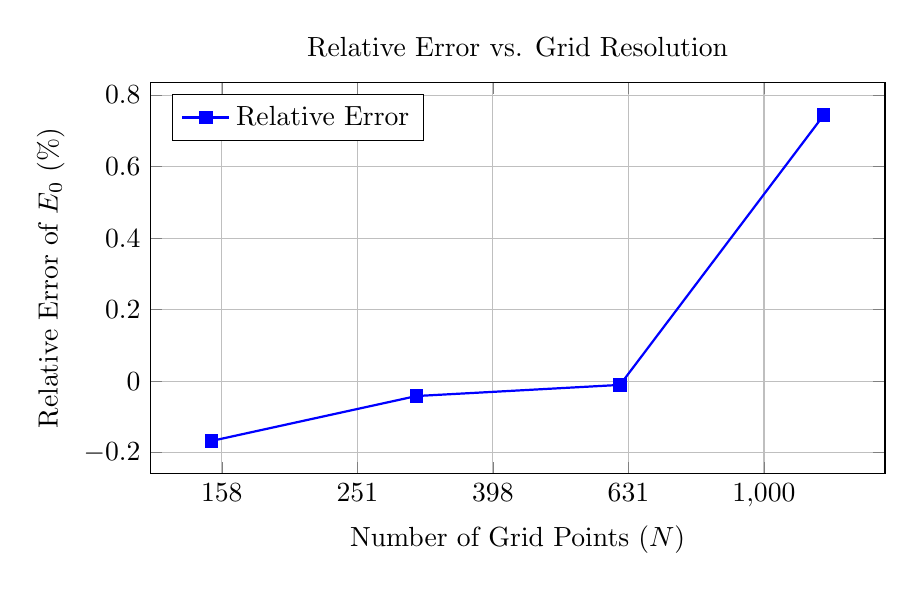
\begin{tikzpicture}
    \begin{axis}[
        width=0.90\textwidth,
        height=0.54\textwidth,
        xlabel={Number of Grid Points ($N$)},
        ylabel={Relative Error of $E_0$ ($\%$)},
        title={Relative Error vs. Grid Resolution},
        grid=both,
        xmode=log,  % Use a logarithmic scale for N since values roughly double
        log ticks with fixed point,
        y tick label style={/pgf/number format/fixed},
        legend pos=north west,
    ]
    \addplot[
        color=blue,
        mark=square*,
        thick,
    ]
    coordinates {
        (153, -0.1671)
        (307, -0.0415)
        (613, -0.0104)
        (1225, 0.7440)
    };
    \addlegendentry{Relative Error}
    \end{axis}
\end{tikzpicture}
\caption{Relative Error vs. Grid Resolution}
\label{fig:relative_error_vs_grid_resolution}
\end{figure}

\section{Parallel Implementation}
\subsection{Parallel Implementation on Google Colab}

The parallel implementation on Google Colab leverages MPI-based domain decomposition for the Lanczos algorithm \cite{10.5555/248511}. The code, written in Python with \texttt{mpi4py}, distributes the computational domain across MPI processes and employs non-blocking communication to exchange ghost cells between neighbouring processes. The Hamiltonian operator is evaluated using finite differences for the kinetic term and a power-law formulation for the potential term.

For the performance evaluation, the algorithm was executed for a fixed physical domain $(L = 25.0)$, a constant Krylov subspace size $(m = 90)$ while varying the number of spatial grid points $N$ (specifically, $N = 513, 1025, \text{and} \; 2049$). Experiments were conducted on three different runtime types available on Colab: CPU, GPU, and TPU. Table~\ref{tab:colab_times} summarizes representative execution times, and Figure~\ref{fig:execution_time_colab} illustrates the trend in execution time as a function of grid resolution.

\begin{table}[h]
    \centering
    \caption{Execution Times ($seconds$) on Google Colab for varying Grid Resolutions ($N$) and Runtime Types}
    \label{tab:colab_times}
    \begin{tabular}{cccc}
    \hline
    $N$ & $CPU \; Time$ & $GPU \; Time$ & $TPU \; Time$ \\ \hline
    $513$   & $11.8043$    & $9.9576$     & $4.0810$    \\
    $1025$  & $14.4722$    & $10.8169$    & $4.7400$    \\
    $2049$  & $15.2353$    & $11.2835$    & $6.4638$    \\ \hline
    \end{tabular}
\end{table}

\begin{figure}[htbp]
\centering
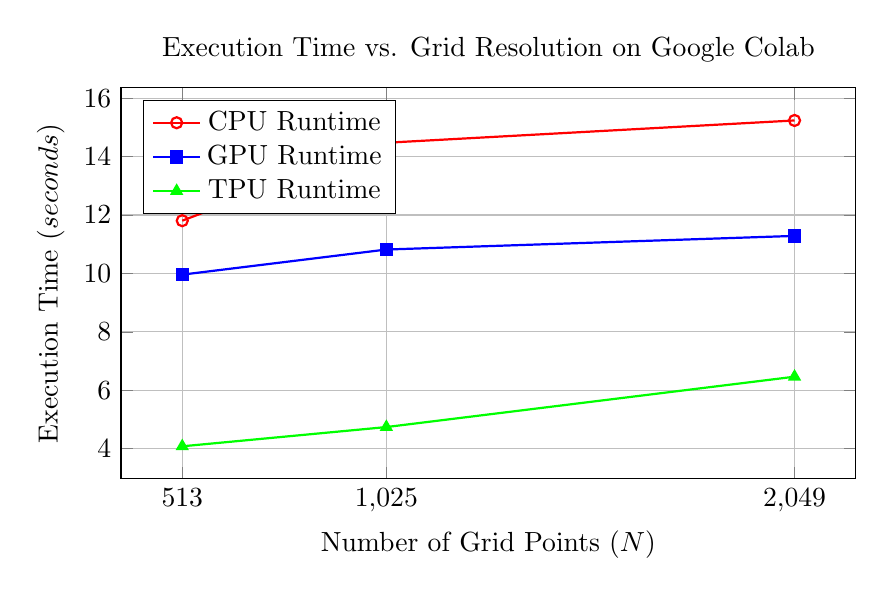
\begin{tikzpicture}
\begin{axis}[
    width=0.90\textwidth,
    height=0.54\textwidth,
    xlabel={Number of Grid Points ($N$)},
    ylabel={Execution Time ($seconds$)},
    title={Execution Time vs. Grid Resolution on Google Colab},
    legend pos=north west,
    grid=both,
    xtick={513,1025,2049},
]
\addplot[
    color=red,
    mark=o,
    thick,
]
coordinates {
    (513,11.8043)
    (1025,14.4722)
    (2049,15.2353)
};
\addlegendentry{CPU Runtime}

\addplot[
    color=blue,
    mark=square*,
    thick,
]
coordinates {
    (513,9.9576)
    (1025,10.8169)
    (2049,11.2835)
};
\addlegendentry{GPU Runtime}

\addplot[
    color=green,
    mark=triangle*,
    thick,
]
coordinates {
    (513,4.0810)
    (1025,4.7400)
    (2049,6.4638)
};
\addlegendentry{TPU Runtime}
\end{axis}
\end{tikzpicture}
\caption{Execution time as a function of the grid resolution for three different runtime types on Google Colab. The TPU runtime achieves the fastest performance, followed by the GPU and CPU runtimes.}
\label{fig:execution_time_colab}
\end{figure}

The results indicate that for a constant physical domain and fixed Krylov subspace size, increasing the number of grid points (i.e., refining the spatial resolution) leads to a moderate increase in execution time on the CPU and GPU. On the other hand, TPU exhibits a more pronounced impact at the highest resolution. Notably, the TPU—with its $8-$core accelerator architecture (totaling $96$ cores)—significantly outperforms the CPU ($2$ cores) and GPU ($2$ cores) implementations. These observations provide valuable insights into the performance characteristics of the MPI-only parallel implementation across the different hardware accelerators available on Google Colab.

\subsection{Parallel Implementation on Stromboli Cluster}

The parallel implementation on the Stromboli Cluster employs a hybrid MPI$+$OpenMP approach to accelerate the Lanczos algorithm for one-dimensional quantum mechanics. In this implementation, the computational domain is partitioned across MPI processes. At the same time, performance‐critical kernels—namely, the Hamiltonian operator and the Modified Gram–Schmidt orthogonalization—are optimized in C using OpenMP directives. The MPI-based domain decomposition efficiently manages inter-process communication (including ghost cell exchanges), and the OpenMP kernels provide additional acceleration on each node.

The code is organized in the file \texttt{matrix\_qm\_parallel\_mpi\_omp.py}, which interfaces with the optimized C/OpenMP library (\texttt{lanczos\_openmp.so}). A substantial scaling study was performed on the Stromboli Cluster by fixing the total problem size (grid points $N$) and the Krylov subspace size $m$ while varying the number of MPI processes from $2$ to $64$. The SLURM script (\texttt{submit\_strong.sh}) automates job submission with varying process counts. Execution times were recorded for several grid sizes (e.g., $N = 32769, 65537, \ldots, 4194305$) and different values of $m \; (\text{e.g.,} \; m=30, 45, 60, \text{and} \; 75)$.

Figure~\ref{fig:stromboli_speedup_fixed_m} shows an illustrative strong scaling plot for the representative case with $m=60$ and $N=524289$. Here, the measured speedup is defined as the ratio of the execution time at $2$ processes to that at a higher process count. For comparison, the ideal speedup—assumed to be $p/2$ (based on the $2-$process baseline)—is also plotted. The results indicate that the measured speedup closely approaches the ideal trend, with only minor deviations at higher processor counts, primarily due to increased communication overhead and node-level load imbalance.
\begin{figure}[htbp]
\centering
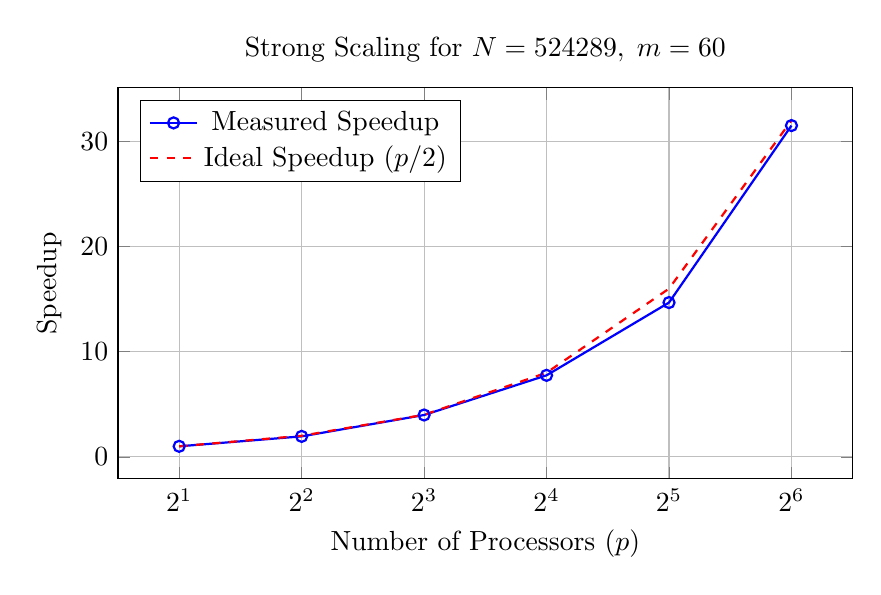
\begin{tikzpicture}
\begin{axis}[
    width=0.90\textwidth,
    height=0.54\textwidth,
    xlabel={Number of Processors ($p$)},
    ylabel={Speedup},
    title={Strong Scaling for $N=524289,\; m=60$},
    xmode=log,
    log basis x=2,
    xtick={2,4,8,16,32,64},
    legend pos=north west,
    grid=both,
]
\addplot[
    color=blue,
    mark=o,
    thick,
]
coordinates {
    (2, 1)
    (4, 1.9457)
    (8, 3.9785)
    (16, 7.7536)
    (32, 14.6749)
    (64, 31.5134)
};
\addlegendentry{Measured Speedup};

\addplot[
    color=red,
    dashed,
    thick,
]
coordinates {
    (2,1)
    (4,2)
    (8,4)
    (16,8)
    (32,16)
    (64,32)
};
\addlegendentry{Ideal Speedup $(p/2)$};
\end{axis}
\end{tikzpicture}
\caption{Strong scaling performance for $m=60$ and $N=524289$ on the Stromboli Cluster}
\label{fig:stromboli_speedup_fixed_m}
\end{figure}

To better understand the sensitivity of scalability to the Krylov subspace size $m$, Figure~\ref{fig:stromboli_common_n_diff_m} compares strong scaling performance at a fixed problem size $N = 131073$ across varying $m = 30, 45, 60, \text{and} \; 75$. The results reveal diverse scaling trends:  
\begin{itemize}
    \item For $m=30$, the speedup curve shows early saturation and deviates significantly from ideal scaling, likely due to insufficient computational workload per process,
    \item For $m=45$ and $m=60$, the scaling improves and aligns more closely with the ideal trend,
    \item For $m=75$, the measured speedup briefly surpasses the ideal speedup—possibly due to favourable cache effects or temporal variability in node performance—but ultimately flattens.
\end{itemize}

\begin{figure}[htbp]
\centering
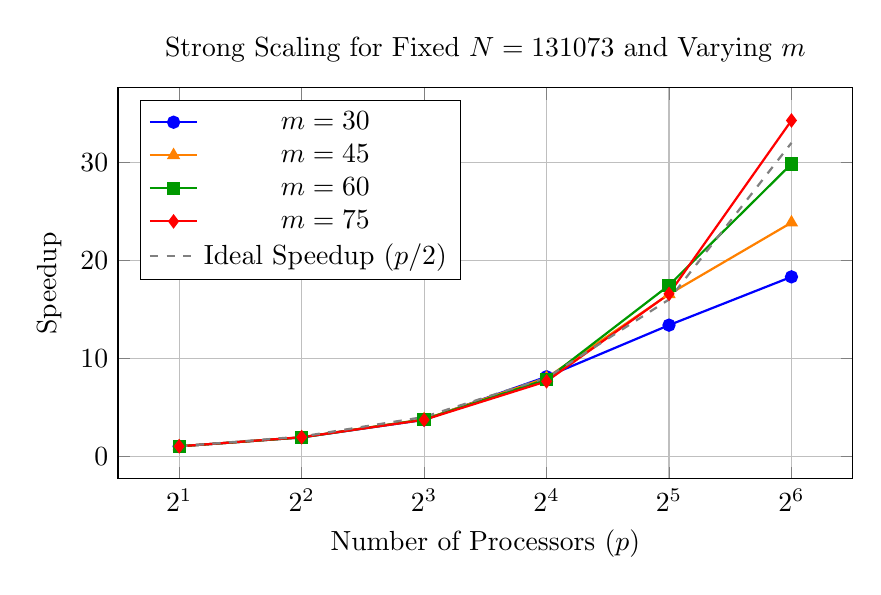
\begin{tikzpicture}
\begin{axis}[
    width=0.90\textwidth,
    height=0.54\textwidth,
    xlabel={Number of Processors $(p)$},
    ylabel={Speedup},
    title={Strong Scaling for Fixed $N=131073$ and Varying $m$},
    xmode=log,
    log basis x=2,
    xtick={2,4,8,16,32,64},
    legend pos=north west,
    grid=both,
]
\addplot[color=blue,mark=*,thick] coordinates {(2,1)(4,1.9114)(8,3.7069)(16,8.1108)(32,13.3788)(64,18.3124)};
\addlegendentry{$m=30$}

\addplot[color=orange,mark=triangle*,thick] coordinates {(2,1)(4,1.9172)(8,3.7574)(16,7.9890)(32,16.5365)(64,23.8549)};
\addlegendentry{$m=45$}

\addplot[color=green!60!black,mark=square*,thick] coordinates {(2,1)(4,1.9113)(8,3.7428)(16,7.8352)(32,17.4462)(64,29.8513)};
\addlegendentry{$m=60$}

\addplot[color=red,mark=diamond*,thick] coordinates {(2,1)(4,1.9302)(8,3.7051)(16,7.6414)(32,16.5731)(64,34.2891)};
\addlegendentry{$m=75$}

\addplot[dashed,color=gray,thick] coordinates {(2,1)(4,2)(8,4)(16,8)(32,16)(64,32)};
\addlegendentry{Ideal Speedup $(p/2)$}
\end{axis}
\end{tikzpicture}
\caption{Speedup comparison for different values of $m$ at fixed $N=131073$}
\label{fig:stromboli_common_n_diff_m}
\end{figure}

Complementarily, Figure~\ref{fig:stromboli_common_m_diff_n} presents strong scaling for fixed $m=30$ over a range of increasing grid sizes $N$. Larger problem sizes exhibit better scalability, as expected, due to an increased compute-to-communication ratio. The lowest grid $(N=32769)$ exhibits early saturation and significant deviation from the ideal trend, whereas for larger grids $(N=131073 \; \text{and above})$, the speedup trend approaches the ideal linear scaling.
\begin{figure}[htbp]
\centering
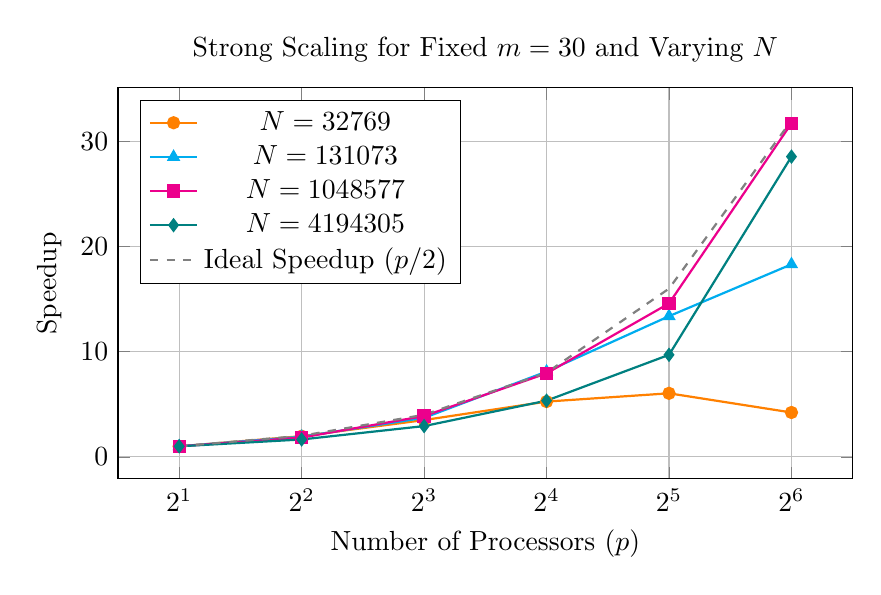
\begin{tikzpicture}
\begin{axis}[
    width=0.90\textwidth,
    height=0.54\textwidth,
    xlabel={Number of Processors $(p)$},
    ylabel={Speedup},
    title={Strong Scaling for Fixed $m=30$ and Varying $N$},
    xmode=log,
    log basis x=2,
    xtick={2,4,8,16,32,64},
    legend pos=north west,
    grid=both,
]
\addplot[color=orange,mark=*,thick] coordinates {(2,1)(4,1.9642)(8,3.4975)(16,5.2549)(32,6.0424)(64,4.2178)};
\addlegendentry{$N=32769$}

\addplot[color=cyan,mark=triangle*,thick] coordinates {(2,1)(4,1.9114)(8,3.7069)(16,8.1108)(32,13.3788)(64,18.3124)};
\addlegendentry{$N=131073$}

\addplot[color=magenta,mark=square*,thick] coordinates {(2,1)(4,1.8308)(8,3.8797)(16,7.9416)(32,14.5933)(64,31.7276)};
\addlegendentry{$N=1048577$}

\addplot[color=green!50!blue,mark=diamond*,thick] coordinates {(2,1)(4,1.6508)(8,2.9243)(16,5.3437)(32,9.7025)(64,28.5604)};
\addlegendentry{$N=4194305$}

\addplot[dashed,color=gray,thick] coordinates {(2,1)(4,2)(8,4)(16,8)(32,16)(64,32)};
\addlegendentry{Ideal Speedup $(p/2)$}
\end{axis}
\end{tikzpicture}
\caption{Speedup comparison for different grid sizes $N$ at fixed $m=30$}
\label{fig:stromboli_common_m_diff_n}
\end{figure}

A consequential aspect of the hybrid implementation is the efficient exchange of boundary data among MPI processes. The function \texttt{exchange\_boundary\_data} performs non-blocking communication to exchange ghost cells between neighbouring processes. Each process maintains a local subdomain augmented with ghost cells at the left and right boundaries. These ghost cells store data from adjacent processes to ensure that finite-difference operations—used in the Hamiltonian operator—can be executed without interruption. This boundary exchange is critical for maintaining data consistency and achieving high parallel efficiency. In particular, for a large computational domain and for the inter-process communication where overhead becomes significant.

To illustrate this mechanism, Figure~\ref{fig:boundary_exchange} depicts a schematic of the domain decomposition. Each row represents the local subdomain of an MPI process (blue cells) sandwiched by ghost cells (orange cells). Arrows indicate the non-blocking communication flow which transfers boundary information between neighbouring processes. Blue arrows represent data sent from the first local cell of a process (e.g., Process $A$ or $B$) to the right ghost cell of its neighbouring process, and red arrows indicate data sent from the last local cell (i.e., the last blue cell) to the left ghost cell of the adjacent process.
\begin{figure}[htbp]
    \centering
    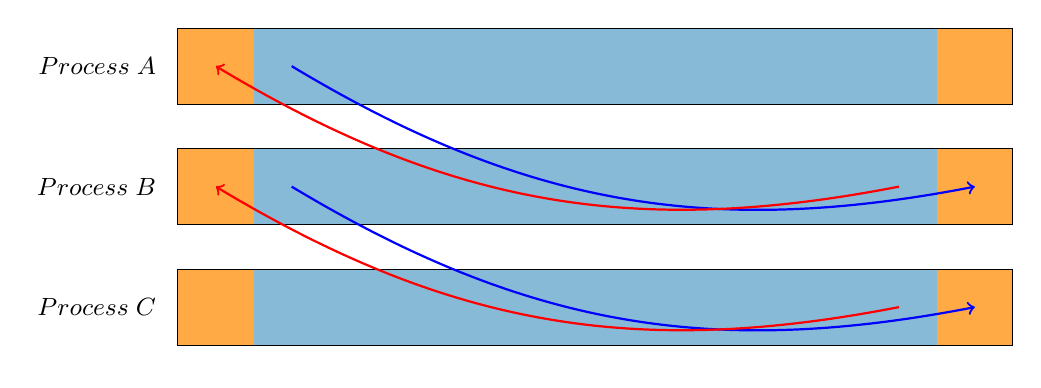
\begin{tikzpicture}[scale=1.53, every node/.style={font=\small}]
        \usetikzlibrary{calc}
        % Define custom colors for ghost and local cells
        \definecolor{ghostColor}{RGB}{255,170,68} % Orange for ghost cells
        \definecolor{localColor}{RGB}{135,186,214} % Blue for local cells
    
        % Configuration parameters
        \def\nCells{9}       % Number of local (blue) cells per process
        \def\cellSize{0.63}  % Width of each cell
    
        % Y-positions for three MPI processes
        \def\yA{2}  % Process A (top)
        \def\yB{1}  % Process B (middle)
        \def\yC{0}  % Process C (bottom)
        
        % Macro to draw one process row with ghost cells
        \newcommand{\drawProcessRow}[2]{
            % Left ghost cell
            \fill[ghostColor] (0, #1) rectangle (\cellSize, {#1+\cellSize});
            % Local (blue) cells; indices 1 to nCells
            \foreach \i in {1,...,\nCells}{
                \fill[localColor] ({\i*\cellSize}, #1) rectangle ({(\i+1)*\cellSize}, {#1+\cellSize});
            }
            % Right ghost cell
            \fill[ghostColor] ({(\nCells+1)*\cellSize}, #1) rectangle ({(\nCells+2)*\cellSize}, {#1+\cellSize});
            % Outline
            \draw[black] (0, #1) rectangle ({(\nCells+2)*\cellSize}, {#1+\cellSize});
            % Label for the process
            \node[anchor=east] at (-0.1, {#1+0.5*\cellSize}) {#2};
        }
        
        % Draw rows for Process A, B, C
        \drawProcessRow{\yA}{$Process \; A$};
        \drawProcessRow{\yB}{$Process \; B$};
        \drawProcessRow{\yC}{$Process \; C$};
        
        % Coordinates for communication points
        % Process A:
        %   First blue cell center: (1.5*cellSize, yA+0.5*cellSize)
        %   Left ghost cell center: (0.5*cellSize, yA+0.5*cellSize)
        \coordinate (A_first) at ($({1.5*\cellSize}, {\yA+0.5*\cellSize})$);
        \coordinate (A_left)  at ($({0.5*\cellSize}, {\yA+0.5*\cellSize})$);
        
        % Process B:
        %   Right ghost cell center: ((nCells+1.5)*cellSize, yB+0.5*cellSize)
        %   Last blue cell center: ((nCells+0.5)*cellSize, yB+0.5*cellSize)
        %   First blue cell center: (1.5*cellSize, yB+0.5*cellSize)
        %   Left ghost cell center: (0.5*cellSize, yB+0.5*cellSize)
        \coordinate (B_right) at ($({(\nCells+1.5)*\cellSize}, {\yB+0.5*\cellSize})$);
        \coordinate (B_last) at ($({(\nCells+0.5)*\cellSize}, {\yB+0.5*\cellSize})$);
        \coordinate (B_first) at ($({1.5*\cellSize}, {\yB+0.5*\cellSize})$);
        \coordinate (B_left)  at ($({0.5*\cellSize}, {\yB+0.5*\cellSize})$);
        
        % Process C:
        %   Right ghost cell center: ((nCells+1.5)*cellSize, yC+0.5*cellSize)
        %   Last blue cell center: ((nCells+0.5)*cellSize, yC+0.5*cellSize)
        %   Left ghost cell center: (0.5*cellSize, yC+0.5*cellSize)
        \coordinate (C_right) at ($({(\nCells+1.5)*\cellSize}, {\yC+0.5*\cellSize})$);
        \coordinate (C_last) at ($({(\nCells+0.5)*\cellSize}, {\yC+0.5*\cellSize})$);
        \coordinate (C_left)  at ($({0.5*\cellSize}, {\yC+0.5*\cellSize})$);
        
        % Draw arrows between Process A and Process B:
        % From Process A's first blue cell to Process B's right ghost cell (blue arrow)
        \draw[->, thick, blue] (A_first) to[bend right=21] (B_right);
        % From Process B's last blue cell to Process A's left ghost cell (red arrow)
        \draw[->, thick, red] (B_last) to[bend left=21] (A_left);
        
        % Draw arrows between Process B and Process C:
        % From Process B's first blue cell to Process C's right ghost cell (blue arrow)
        \draw[->, thick, blue] (B_first) to[bend right=21] (C_right);
        % From Process C's last blue cell to Process B's left ghost cell (red arrow)
        \draw[->, thick, red] (C_last) to[bend left=21] (B_left);

    \end{tikzpicture}
    \caption{Schematic illustration of boundary exchange in the hybrid MPI$+$OpenMP implementation. Each MPI process holds its local subdomain (blue cells) and ghost cells (orange) at the boundaries. Blue arrows represent data sent from the first local cell of a process (e.g., Process $A$ or $B$) to the right ghost cell of the neighbouring process, while red arrows depict data sent from the last local cell (i.e., the last blue cell) to the left ghost cell of the adjacent process.}
    \label{fig:boundary_exchange}
\end{figure}

These scaling studies indicate that the overall parallel performance depends critically on the Krylov subspace size $m$ and the total number of grid points $N$. Smaller $m$ or $N$ may lead to suboptimal scaling due to limited per-processor workload, conversely, larger values of $m$ and $N$ help sustain near-ideal or even superlinear speedup due to improved parallel efficiency, cache utilization, and reduced relative communication overhead. Overall, these results validate the effectiveness of the hybrid MPI$+$OpenMP strategy for large-scale quantum simulations \cite{Heath2002} on modern HPC architectures.


% Chapter 5: Conclusion and Outlook
\chapter{Conclusion and Outlook}

In this work, we have developed and rigorously validated a numerical framework for solving quantum mechanical eigenvalue problems using a matrix formulation and the Lanczos algorithm. By discretizing the Schrödinger equation for one-dimensional systems, we effectively reduced the continuous problem into a large, sparse matrix eigenvalue problem. This approach was successfully applied to benchmark systems—such as the quantum harmonic oscillator—where the computed eigenvalues show excellent agreement with the analytical solutions.

The serial implementation based on a finite difference discretization combined with full reorthogonalization via the Modified Gram–Schmidt process delivers a robust baseline. Detailed convergence studies demonstrate that the Lanczos algorithm converges rapidly with minimal relative error, confirming its accuracy and efficiency even for large matrix dimensions. Building on this foundation, we extended the numerical framework to a parallel implementation using MPI for inter-process communication. On the Google Colab platform, the MPI-only version displayed significant execution time improvements for varying grid resolutions. The hybrid MPI$+$OpenMP implementation on the Stromboli Cluster achieved nearly ideal strong scaling performance across a range of problem sizes and Krylov subspace dimensions.

A key innovation in our approach is the efficient management of ghost cell exchanges, which ensures consistency in finite-difference operations across process boundaries. Optimizations at both the algorithmic and code levels—such as utilizing OpenMP-accelerated kernels for the Hamiltonian operator and orthogonalization routines—were critical in achieving high computational performance on modern HPC architectures.

\section*{Outlook}

The positive results obtained from our numerical framework suggest several promising directions for future research:
\begin{itemize}
    \item \textbf{Extension to Higher Dimensions:} The current framework is limited to one-dimensional systems. Future work will extend these methods to two- and three-dimensional systems, which will require more advanced discretization strategies and shall pose additional computational challenges.
    
    \item \textbf{Enhanced Parallelization Strategies:} Further improvements in scalability could be achieved by exploring sophisticated load-balancing techniques, hybrid approaches that combine MPI with GPU acceleration, and the emerging hardware paradigms integration.
    
    \item \textbf{Application to Complex Quantum Systems:} The matrix formulation and Lanczos algorithm can be adapted to more intricate potential landscapes and many-body quantum systems. This extension will be significant for studying quantum phase transitions, strongly correlated systems, and quantum dynamics.
    
    \item \textbf{Algorithmic Refinements:} Future work may incorporate adaptive techniques to dynamically adjust the Krylov subspace size and explore alternative reorthogonalization methods to improve accuracy and performance.
    
    \item \textbf{Software Integration and Benchmarking:} Integrating the present framework with established quantum mechanics simulation packages and benchmarking against state-of-the-art methods would further validate its performance and help identify further optimization opportunities.
\end{itemize}

In summary, our work lays a solid foundation for the numerical exploration of quantum systems through efficient matrix methods and scalable parallel implementations. The encouraging results provide a clear pathway for future research, which will broaden the applicability of these techniques to more complex physical systems and computational environments.

\bigskip
\noindent\textbf{Acknowledgements:} First and foremost, we express our sincere gratitude to advisor, \textit{Dr. Tomasz Korzec}, for the opportunity to work on such an engaging project and for his invaluable guidance and continuous support throughout this project. We also acknowledge the Google Colab platform and the computational resources provided by the \textit{Stromboli} cluster at Bergische Universität Wuppertal.


% Appendix
\appendix
\appendixpage

\chapter{Python/MPI Program Code Listings}
\section{Lanczos Algorithm Implementation}
\lstinputlisting[language=Python, linerange={39-39, 57-119}]{./matrix_qm_parallel_mpi_omp.py}
\section{Loading C/OpenMP library \& defining function signatures}
\lstinputlisting[language=Python, linerange={12-14, 16-16, 19-33}]{./matrix_qm_parallel_mpi_omp.py}
\section{MPI Helper Functions}
\lstinputlisting[language=Python, linerange={125-127, 131-137, 150-192}]{./matrix_qm_parallel_mpi_omp.py}
\section{Python wrappers for calling C routines}
\lstinputlisting[language=Python, linerange={198-200, 211-224, 234-244}]{./matrix_qm_parallel_mpi_omp.py}

\chapter{C/OpenMP Program Code Listings}
\section{C Kernel for Hamiltonian Application}
\lstinputlisting[language=C, linerange={14-14, 19-35}]{./lanczos_openmp.c}
\section{C Kernel for Modified Gram-Schmidt}
\lstinputlisting[language=C, linerange={38-38, 46-85}]{./lanczos_openmp.c}

\chapter{Shell Script Listings}
\section{Shell Script for Job Submission}
\lstinputlisting[language=bash, linerange={1-1, 7-62}]{submit_strong.sh}


% Bibliography
\printbibliography[heading=bibintoc]


% End the Document
\end{document}